\documentclass[10pt,a4paper]{amsart}
\usepackage[margin=19mm]{geometry}
\usepackage{amsmath,amssymb,mathtools}
\usepackage[scr=rsfs,cal=euler]{mathalfa}
\usepackage{xfrac}
\usepackage[unicode,hidelinks,bookmarks=false]{hyperref}
\newcommand{\ie}{i.e.\ }
\newcommand{\cf}{cf.\ }
\newcommand{\resp}{respectively\ }
\newcommand{\Subsection}{\subsection}
\providecommand{\nobreakdash}{\nobreak\hbox{-}}
\setlength{\emergencystretch}{2em}
\multlinegap0pt
\usepackage{tikz}
\usepackage{float}
\usepackage{amssymb}
\usepackage{csquotes}
\newtheorem{lem}{Lemma}
\usepackage{cleveref}
\crefname{lem}{Lemma}{Lemmas}
\newcommand{\emphd}[1]{{\fontseries{b}\selectfont\textsf{#1}}}
\title{\vspace{-2cm}The linear Tur\'an number of the 3-graph $P_5$}
\author{Chaoliang Tang, Hehui Wu, Junchi Zhang}
\date{Source: arXiv:2601.19068v1 (CC BY 4.0)}
\begin{document}
\maketitle

\noindent\emph{Source and licence.} \vspace{-2cm}The linear Tur\'an number of the 3-graph $P_5$. Version arXiv:2601.19068v1 (CC BY 4.0), distributed by arXiv under the Creative Commons Attribution 4.0 International licence, http://creativecommons.org/licenses/by/4.0/, as recorded in the arXiv licence metadata for this exact version and shown on the abstract page https://arxiv.org/abs/2601.19068v1. Full licence notice: \texttt{licenses/arxiv-2601.19068-CC-BY-4.0.txt}.\par\smallskip

\noindent\textit{Editorial scope.} Counted unit: the article's lem I3P2 (source0.tex lines 708--710). The article's complete original proof of it is delivered with it (source0.tex lines 711--1053, one \texttt{proof} environment of 343 lines). No mathematics is written, repaired or re-derived: the statement and the proof are the article's own lines, in the article's own notation, and no retained line is substituted or re-flowed.  Retained uncounted as the source-local context the proof needs: lines 440--442; lines 639--645; lines 690--692.  Nothing was omitted from any retained span, so the package carries no omission record.  No retained line contains a citation, so the wrapper carries no bibliography and no bibliography entry.  The retained lines contain the article's own diagram code, which the wrapper typesets with the standard tikz packages; no image file is delivered and the package declares no asset dependency.  Editorial formatting only, in addition: an AMS \texttt{amsart} preamble that restates the article's own declarations and macros used by the retained lines, namely the environments \texttt{lem} on separate counters, together with the standard packages those lines need.  The retained environments print in this document as Lemma 1 in order of appearance, whereas the article prints the same items with the numbering of its own full document.  The complete native source of the article as distributed in the arXiv e-print for this exact version is bundled unchanged as \texttt{sources/193437/source0.tex}.
\begin{lem}\label{contradiction}
    For any vertex set $S\subseteq G$, $|E(S)| \ge \frac{15}{11}|S|$. In particular, $\delta(G)\ge 2$.
\end{lem}

\begin{lem}\label{conpath}
    Let $U,V$ be two disjoint connected subgraphs of $G$, and $P$ is a path connecting $U$ and $V$ which does not contain a center of $U$ or $V$. Then one of the following holds.
    \begin{enumerate}
    \item $P$ is an edge and consists of a 2-center of one of $U,V$ and a center pair of the other.
    \item $P$ is a path of length 2 and $P\cap U, P\cap V$ are center pairs of $U,V$ respectively.
    \end{enumerate}
\end{lem}

\begin{lem}\label{4P2}
	For $U=P_4$ or $C_4$, there is no disjoint $U$ and $P_2$ in $G$.
\end{lem}

\begin{lem}\label{I3P2}
	After deleting the vertices of an arbitrary $P_2$ in $G$, if some component contains a $P_3$, then this component is exactly a $P_3$. 
\end{lem}

\begin{proof}
Suppose after deleting vertices of some subgraph $V=P_2$ in $G$ consisting of two edges $v_1v_2v_3, v_3v_4v_5$, there is a component containing a $P_3$ but not a $P_3$ by itself. By~\Cref{4P2}, it does not contain a $P_4$ or $C_4$ and thus the component contains a subgraph $U=L_{14},L_{11},L_{12},L_{8}$ or $L_{13}$.
    
(1) $U=L_{14}$.
    \begin{figure}[h]
	\centering
	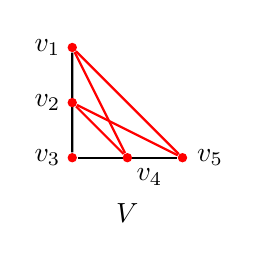
\begin{tikzpicture}[scale=0.7, every node/.style={circle, fill, inner sep=1.2pt}]
		\node[fill=red] (v1) at (-1, 0) {};
		
		\node[fill=red] (v3) at (1, 0) {};
		
		\node[fill=red] (v5) at (-1, 2) {};

		
		\draw[black, thick] (v1) -- (v3);
		\draw[black, thick] (v1) -- (v5);
		
        
        \node[fill=red] (v4) at (-1, 1) {};
		\node[fill=red] (v2) at (0, 0) {};
        \draw[red, thick] (v3) -- (v4);
		\draw[red, thick] (v2) -- (v5);
		\draw[red, thick] (v3) -- (v5);
		\draw[red, thick] (v2) -- (v4);

		\node[draw=none,fill=none] at (-1.45, 2) {$v_1$};
		\node[draw=none,fill=none] at (-1.45, 1) {$v_2$};
		\node[draw=none,fill=none] at (-1.45, 0) {$v_3$};
		\node[draw=none,fill=none] at (0.4, -0.35) {$v_4$};
		\node[draw=none,fill=none] at (1.5, 0) {$v_5$};
		\node[draw=none,fill=none] at (0, -1) {$V$};
		
	\end{tikzpicture}%
    \hspace{0.4cm}
	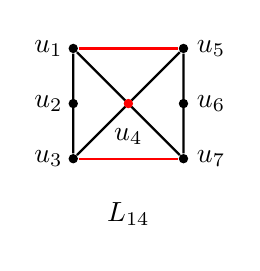
\begin{tikzpicture}[scale=0.7, every node/.style={circle, fill, inner sep=1.2pt}]
	\node[fill=black] (v1) at (-1, 0) {};
	\node[fill=black] (v3) at (1, 0) {};
	\node[fill=black] (v4) at (-1, 1) {};
	\node[fill=black] (v5) at (-1, 2) {};
	\node[fill=black] (v6) at (1, 1) {};
	\node[fill=black] (v7) at (1, 2) {};	
	\node[draw=none,fill=none] at (-1.45, 2) {$u_1$};
	\node[draw=none,fill=none] at (-1.45, 1) {$u_2$};
	\node[draw=none,fill=none] at (-1.45, 0) {$u_3$};
	\node[draw=none,fill=none] at (0, 0.4) {$u_4$};
	\node[draw=none,fill=none] at (1.5, 2) {$u_5$};
	\node[draw=none,fill=none] at (1.5, 1) {$u_6$};
	\node[draw=none,fill=none] at (1.5, 0) {$u_7$};
	
	\draw[black, thick] (v1) -- (v7);
	\draw[black, thick] (v1) -- (v5);
	\draw[black, thick] (v3) -- (v5);
	\draw[black, thick] (v3) -- (v7);
		\node[fill=red] (v2) at (0, 1) {};
	\draw[red, thick] (v1) -- (v3);
	\draw[red, thick] (v5) -- (v7);
	\node[draw=none,fill=none] at (0, -1) {$L_{14}$};
	
\end{tikzpicture}	
\end{figure}

	In the figure above, we color the 2-centers red and connect the center pairs by red edges in $U$ and $V$. Let $S=V(U)-u_4$, $F_U$ be the 4 edges in $U$, $E^-(S) =E(S)-F_U-E(v_3)$ and $E_i^-(S) = E_i(S)-F_U-E(v_3)$ for $i=1,2,3$. Note that $E_3^-(S)=\emptyset$ by linearity, and thus $E^-(S) = E_1^-(S)\cup E_2^-(S)$. 
    
    By~\Cref{contradiction}, $|E(S)|\ge 9$, which means $|E^-(S)|+|E(v_3)\cap E(S)|\ge 5$. Our goal is to show that $|E^-(S)|+|E(v_3)\cap E(S)|\leq 4$ and obtain a contradiction. 

    For $g\in E_1^-(S)$, we claim that $u_4\in g$. If not, by symmetry we can assume $g\cap U\in\{u_1,u_2\}$. Then either $g,u_1u_2u_3,u_3u_4u_5,u_5u_6u_7$ form a $P_4$ disjoint from $V$, contradicting~\Cref{4P2},
    or there exists $g'\in\{v_1v_2v_3,v_3v_4v_5\}$ such that $g',g,u_1u_2u_3,u_3u_4u_5,u_5u_6u_7$ form a $P_5$ in $G$, a contradiction. Moreover, by linearity $u_1,u_3,u_5,u_7\notin g$, so $g\cap U\in \{u_2,u_6\}$. Since $g\notin E(v_3)$, if $g\cap V\neq \emptyset$, by symmetry we can assume $g=v_1u_2u_4$, 
    and then $v_5v_4v_3,v_3v_2v_1,v_1u_2u_4,u_4u_3u_5,u_5u_6u_7$ form a $P_5$ in $G$, a contradiction. In conclusion, for any $g\in E_1^-(S)$, $g=u_4u_2u_8$ or $u_4u_6u_9$, where $u_8$ and $u_9$ lie outside $U\cup V$. Since there is no $P_4$ disjoint from $V$, these two edges cannot exist simultaneously. Thus $|E_1^-(S)|\le 1$.

    For $g\in E(S)\cap E(v_3)$, by linearity $|g\cap V|=1$ and $g$ connects $V,U$. If $|g\cap U|=1$, since any vertex in $S$ is an endpoint of a $P_3$ in $U$, there exists a $P_5$ in $G$ consisting of this $P_3$ and $g, v_1v_2v_3$, a contradiction. Thus $|g\cap U|=2$, and by linearity we have $|E(S)\cap E(v_3)|\le \lfloor\frac{|U|}{2}\rfloor=3$.

     Let $E'$ be the set of edges in $E^-(S)$ containing a center pair of $U$, i.e., containing either $u_3u_7$ or $u_1u_5$.
    
    \emphd{Case 1.} $E'=\emptyset$. Since $|E(S)\cap E(v_3)|\le 3$, it suffices to show $|E_2^-(S)\cup E_1^-(S)|\le 1$.
    
    For $h \in E_2^-(S)$, by definition $v_3\notin h$, and by symmetry, we could suppose $h\cap S=u_1u_6$ or $u_2u_6$. Immediately we obtain that the third vertex $w= h-S\in U\cup V$ since otherwise $u_1u_2u_3,u_3u_4u_5,u_5u_6u_7,h$ is a $C_4$ disjoint from $V$, contradicting~\Cref{4P2}. If $w\in V$, then by definition, $w\neq v_3$, and by symmetry, we can assume $w=v_1$ and then $v_5v_4v_3,v_3v_2v_1,h,u_6u_5u_7,u_5u_4u_3$ forms a $P_5$, a contradiction. Thus, $w=u_4$ because $w\notin S$. By linearity, the only possible case of $h$ is $u_4u_2u_6$, which implies that $E_2^-(S)\subseteq\{u_4u_2u_6\}$. Again by linearity, any two of $u_2u_4u_6,u_2u_4u_8$ and $u_4u_6u_9$ cannot exist simultaneously, which implies that $|E_2^-(S)\cup E_1^-(S)|\le 1$. 

	\emphd{Case 2.} $|E'|=1$. By symmetry, we can assume $E'=\{u_1 u_5 w\}$. It suffices to show $|E_2^-(S)\cup E_1^-(S)|\le 1$.

    As the discussion in Case 1, $E_2^-(S)\subseteq E' \cup\{u_4u_2u_6\}$. If $u_4u_2u_6$ is an edge of $G$, then $w\notin U\cup V$, since otherwise $h,u_1u_2u_3,u_2u_4u_6,u_6u_7u_5$ is a $C_4$ disjoint from $V$, a contradiction. Further as in Case 1, we have $E_1^-(S)=\emptyset$, and thus $|E_2^-(S)\cup E_1^-(S)|\le 1$. So we can assume $E_2^-(S)=E'$.
    
    If $w\in U\cup V$, then by definition $w\in V-v_3$, and by symmetry we can assume $w=v_1$. If there is an edge $g\in E_1^-(S)$, by symmetry we can assume $g=u_2u_4w'$ such that $w'\notin U\cup V$. Then $v_5v_4v_3,v_3v_2v_1,h,u_1u_2u_3,g$ is a $P_5$ in $G$, a contradiction.
    
    If $w\notin U\cup V$, we claim that there exists no edge $g=u_2u_4w'$ or $u_4u_6w'$ such that $w'\notin U\cup V$. If not, and if $w\neq w'$, then we can find a $P_4$ disjoint from $V$, a contradiction. By symmetry and linearity we can assume $w=w'$, $g=wu_2u_4\in E (G)$ and $wu_4u_6\notin G$. Then we have $h'=v_3u_3u_6$ or $v_3u_3u_7 \notin E (G)$, otherwise $v_1v_2v_3,h',u_7u_6u_5,u_5u_1w,wu_2u_4$ is a $P_5$ in $G$, a contradiction. 
    Thus $E(S)\cap E(v_3)\subseteq\{v_3u_1u_6,v_3u_2u_5,v_3u_2u_6,v_3u_2u_7\}$. By linearity, $|E(S)\cap E(v_3)|\leq 2$. Note that by the above discussion edges in $E_1^-(S)$ contains $u_4$ and thus $|E^-(S)|\leq 2$. Then we have $|E^-(S)|+|E(v_3)\cap E(S)|\le 4$, a contradiction.
    Thus we have $E_1^-(S)=\emptyset$ and $|E_2^-(S)\cup E_1^-(S)|=1$.
    
	\emphd{Case 3.} $|E'|=2$. As the discussion in case 2, $E_2^-(S)=E'$ and $E_1^-(S)=\emptyset$. Thus for any edge in $E^-(S)\cap E(v_3)$, it must contain one of $u_2,u_4$ by linearity. We conclude that $|E^-(S)|+|E(v_3)\cap E(S)|\le 4$.\\
    
	(2) $U=L_{11}$.
        \begin{figure}[h]
	\centering
	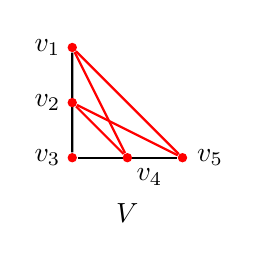
\begin{tikzpicture}[scale=0.7, every node/.style={circle, fill, inner sep=1.2pt}]
		\node[fill=red] (v1) at (-1, 0) {};
		
		\node[fill=red] (v3) at (1, 0) {};
		
		\node[fill=red] (v5) at (-1, 2) {};
		
        
		
		\draw[black, thick] (v1) -- (v3);
		\draw[black, thick] (v1) -- (v5);
        \node[fill=red] (v4) at (-1, 1) {};
		\node[fill=red] (v2) at (0, 0) {};
        
		\draw[red, thick] (v3) -- (v4);
		\draw[red, thick] (v2) -- (v5);
		\draw[red, thick] (v3) -- (v5);
		\draw[red, thick] (v2) -- (v4);


		\node[draw=none,fill=none] at (-1.45, 2) {$v_1$};
		\node[draw=none,fill=none] at (-1.45, 1) {$v_2$};
		\node[draw=none,fill=none] at (-1.45, 0) {$v_3$};
		\node[draw=none,fill=none] at (0.4, -0.35) {$v_4$};
		\node[draw=none,fill=none] at (1.5, 0) {$v_5$};
		\node[draw=none,fill=none] at (0, -1) {$V$};
		
	\end{tikzpicture}%
    \hspace{0.4cm}
	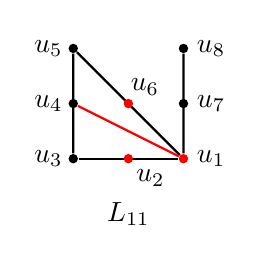
\begin{tikzpicture}[scale=0.7, every node/.style={circle, fill, inner sep=1.2pt}]
	\node[fill=black] (v1) at (-1, 0) {};

	\node[fill=red] (v3) at (1, 0) {};
	\node[fill=black] (v4) at (-1, 1) {};
	\node[fill=black] (v5) at (-1, 2) {};

	\node[fill=black] (v8) at (1, 1) {};
	\node[fill=black] (v9) at (1, 2) {};

	
	\draw[black, thick] (v1) -- (v3);
	\draw[black, thick] (v1) -- (v5);
	\draw[black, thick] (v3) -- (v5);
	\draw[black, thick] (v3) -- (v9);
	\draw[red, thick] (v4) -- (v3);
		\node[fill=red] (v2) at (0, 0) {};
		\node[fill=red] (v6) at (0, 1) {};
		\node[draw=none,fill=none] at (-1.45, 2) {$u_5$};
	\node[draw=none,fill=none] at (-1.45, 1) {$u_4$};
	\node[draw=none,fill=none] at (-1.45, 0) {$u_3$};
	\node[draw=none,fill=none] at (0.4, -0.35) {$u_2$};
	\node[draw=none,fill=none] at (0.3, 1.3) {$u_6$};
	\node[draw=none,fill=none] at (1.5, 2) {$u_8$};
	\node[draw=none,fill=none] at (1.5, 1) {$u_7$};
	\node[draw=none,fill=none] at (1.5, 0) {$u_1$};
	\node[draw=none,fill=none] at (0, -1) {$L_{11}$};
\end{tikzpicture}	
\end{figure}

Let $S = \{u_7, u_8\}$, $T = \{v_1, v_2, v_4, v_5\}$. For any $h\in E_1(S)$, by~\Cref{4P2} and (1) we have $h\cap V \neq \emptyset$, and thus $h$ connects $U,V$. 
Since $u_7, u_8$ are not 2-centers or vertices of center pairs, by~\Cref{conpath} $h\cap V = \{v_3\}$. Let $\tilde{v} = h-\{u_7,u_8,v_3\}$. If $\tilde{v}\notin U$, then $e_1, h, u_1u_7u_8, u_1u_2u_3, u_3u_4u_5$ form a $P_5$. Thus $\tilde{v}\in U$. Observe that $\tilde{v}\neq u_1$ by linearity. If $\tilde{v}=u_2$, then $u_3u_4u_5,u_5u_6u_1,u_1u_7u_8,h,v_3v_2v_1$ form a $P_5$. So $\tilde{v}\not=u_2$ and by symmetry $\tilde{v}\not=u_6$. Hence $\tilde{v}\in \{u_3,u_4, u_5\}$. By~\Cref{contradiction} with $|S|=2$, we have $|E_1(S)|\ge 2$. So we can choose some $h\in E_{1}(S)$ such that $\tilde{v}\not=u_4$. By symmetry we can assume $h=u_8u_3v_3$.
	
By~\Cref{contradiction}, $|E(T)|\geq 6$. First, $|E_3(T)|=0$ by linearity. Next, note that $u_5u_6u_1,u_1u_2u_3,u_3u_8v_3$ and $v_1v_2v_3(v_3v_4v_5)$ already form a $P_4$. This implies that every edge $e$ in $E(T)-\{v_1v_2v_3,v_3v_4v_5\}$ connects $V$ and $U$. Thus by~\Cref{conpath}, $e$ must contain the only center pair $u_1u_4$ of $U$. So $|E_1(T)|\le 1$ and thus $|E_2(T)|\ge 5$.
	
For any edge $g\in E_2(T)-\{v_1v_2v_3,v_3v_4v_5\}$, let $\tilde{u}=g-T$.
If $u\notin U$, then $g,v_1v_2v_3,h,u_8u_7u_1,u_1u_6u_5$ form a $P_5$ in $G$, a contradiction. Thus $g$ connects $U,V$ and by~\Cref{conpath}, $\tilde{u}\in \{u_1,u_2,u_6\}$. If $\tilde{u}=u_2$, then $u_1u_6u_5,u_5u_4u_3,h,v_1v_2v_3,g$ form a $P_5$, a contradiction. So $\tilde{u}\in\{u_1,u_6\}$. By linearity, there are at most two edges in $E_2(T)$ containing $u_6$ and at most two edges in $E_2(T)$ containing $u_1$. However, $|E_2(T)|\ge 5$, so there exists at least 3 edges in $E_2(T)$ containing one of $u_1$ and $u_6$. So we can find two edges $e_1,e_2\in E_2(S)$ such that $\emptyset \neq e_1\cap e_2\subseteq S$ and $u_1\in e_1$, $u_6\in e_2$. Assume $e_3\in\{v_1v_2v_3,v_3v_4v_5\}$ does not contain $e_1\cap e_2$. Then $e_2,e_1,v_1v_7v_8,h=u_8u_3v_3,e_3$ form a $P_5$, a contradiction.\\
    
(3) $U=L_{12}$.
    
    \begin{figure}[h]
	\centering
	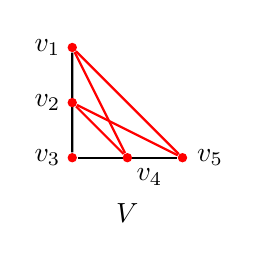
\begin{tikzpicture}[scale=0.7, every node/.style={circle, fill, inner sep=1.2pt}]
		\node[fill=red] (v1) at (-1, 0) {};
		\node[fill=red] (v3) at (1, 0) {};
		\node[fill=red] (v5) at (-1, 2) {};
		\draw[black, thick] (v1) -- (v3);
		\draw[black, thick] (v1) -- (v5);
        \node[fill=red] (v4) at (-1, 1) {};
		\node[fill=red] (v2) at (0, 0) {};
		\draw[red, thick] (v3) -- (v4);
		\draw[red, thick] (v2) -- (v5);
		\draw[red, thick] (v3) -- (v5);
		\draw[red, thick] (v2) -- (v4);

		\node[draw=none,fill=none] at (-1.45, 2) {$v_1$};
		\node[draw=none,fill=none] at (-1.45, 1) {$v_2$};
		\node[draw=none,fill=none] at (-1.45, 0) {$v_3$};
		\node[draw=none,fill=none] at (0.4, -0.35) {$v_4$};
		\node[draw=none,fill=none] at (1.5, 0) {$v_5$};
		\node[draw=none,fill=none] at (0, -1) {$V$};
		
	\end{tikzpicture}%
    \hspace{0.4cm}
	\begin{tikzpicture}[scale=0.7, every node/.style={circle, fill, inner sep=1.2pt}]
	\node[fill=red] (v1) at (-1, 0) {};

	\node[fill=red] (v3) at (1, 0) {};
	\node[fill=black] (v4) at (-1, 1) {};
	\node[fill=black] (v5) at (-1, 2) {};
	\node[fill=black] (v6) at (1, 1) {};
	\node[fill=black] (v7) at (1, 2) {};
	\node[fill=black] (v8) at (-0.5, 1) {};

	
	\draw[black, thick] (v1) -- (v3);
	\draw[black, thick] (v1) -- (v5);
	\draw[black, thick] (v3) -- (v7);
	\draw[black, thick] (v5) -- (v2);
	\draw[red, thick] (v3) -- (v5);
	\node[fill=red] (v2) at (0, 0) {};
		\node[draw=none,fill=none] at (-1.45, 2) {$u_5$};
		\node[draw=none,fill=none] at (-1.45, 1) {$u_4$};
		\node[draw=none,fill=none] at (-1.45, 0) {$u_3$};
		\node[draw=none,fill=none] at (0.4, -0.35) {$u_1$};
		\node[draw=none,fill=none] at (-0.1, 0.65) {$u_6$};
		\node[draw=none,fill=none] at (1.5, 2) {$u_8$};
		\node[draw=none,fill=none] at (1.5, 1) {$u_7$};
		\node[draw=none,fill=none] at (1.5, 0) {$u_2$};
	\node[draw=none,fill=none] at (0, -1) {$L_{12}$};
\end{tikzpicture}	
\end{figure}

Let $S = \{u_7, u_8\}$, $T = \{v_1, v_2,v_4,v_5\}$.	If there is no edge $\tilde{u}_1\tilde{u}_2v_3$ such that $\tilde{u}_1\in \{u_7, u_8\}, \tilde{u}_2\in\{u_1, u_3\}$, we claim that $|E_1(S)|\le 1$. For any $h\in E_1(S)$,  by~\Cref{4P2} and case (1) we have $h\cap V \neq \emptyset$. It follows that $h\cap V = \{v_3\}$ since $u_7, u_8$ are not 2-centers or vertices of center pair. 
Let $\tilde{v} = h-\{u_7,u_8,v_3\}$, then $\tilde{v}\notin \{u_1, u_3\}$ by our assumption and $\tilde{v}\neq u_2$ by linearity. If $\tilde{v}=u_4$, then $u_5u_6u_1, u_1u_3u_2,u_2u_7u_8, h, v_3v_2v_1$ form a $P_5$. So $\tilde{v}\neq u_4$ and $\tilde{v}\neq u_6$ by symmetry. Thus $\tilde{v} = u_5$ and $|E_1(S)|\le 1$ by linearity. Thus $|E(S)|\leq 2<\frac{15}{11}|S|$, contradicting~\Cref{contradiction}.
	
Now by symmetry, we can assume $h =u_8v_3u_1\in E (G)$. Our goal compute $|E(T)|$. To start with, $|E_3(T)|=0$ by linearity. Next, note that $u_3u_4u_5,u_5u_6u_1,h=u_1u_8v_3$ and $e_1$ or $e_2$ already form a $P_4$. This implies that every edge in $E(T)-\{v_1v_2v_3,v_3v_4v_5\}$ connects $V$ and $U$, a star and a non-star subgraph. Thus by~\Cref{conpath},
for any edge in $E_1(T)$, it must the only center pair $u_2u_5$ of $U$, and thus $|E_1(T)|\le 1$. 
For any edge $g\in E_2(T)-\{v_1v_2v_3,v_3v_4v_5\}$, let $\tilde{u}=g-T$ and again by~\Cref{conpath}, $\tilde{u}$ has to be a 2-center in $U$. So $\tilde{u}\in \{u_1,u_2,u_3\}$. If $\tilde{u}=u_2$, then $u_3u_4u_5,u_5u_6u_1,h=u_8v_3u_1,v_1v_2v_3,g$ form a $P_5$, a contradiction. If $\tilde{u} = u_3$, then $u_2u_7u_8, h=u_8u_1v_3, v_3v_2v_1, g, u_3u_4u_5$ form a $P_5$, a contradiction. So $\tilde{u} = u_1$, which implies that $|E_2(T)-\{e_1,e_2\}|\le 2$ by linearity. Therefore, $|E(T)|\le 5<\frac{15}{11}|T|$, contradicting~\Cref{contradiction}.\\
    
	(4) $U=L_8$.
     \begin{figure}[h]
	\centering
	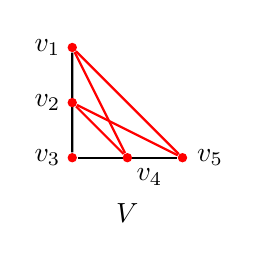
\begin{tikzpicture}[scale=0.7, every node/.style={circle, fill, inner sep=1.2pt}]
		\node[fill=red] (v1) at (-1, 0) {};
		\node[fill=red] (v3) at (1, 0) {};
		\node[fill=red] (v5) at (-1, 2) {};
		
		
		\draw[black, thick] (v1) -- (v3);
		\draw[black, thick] (v1) -- (v5);
        \node[fill=red] (v4) at (-1, 1) {};
		\node[fill=red] (v2) at (0, 0) {};
        
		\draw[red, thick] (v3) -- (v4);
		\draw[red, thick] (v2) -- (v5);
		\draw[red, thick] (v3) -- (v5);
		\draw[red, thick] (v2) -- (v4);

		\node[draw=none,fill=none] at (-1.45, 2) {$v_1$};
		\node[draw=none,fill=none] at (-1.45, 1) {$v_2$};
		\node[draw=none,fill=none] at (-1.45, 0) {$v_3$};
		\node[draw=none,fill=none] at (0.4, -0.35) {$v_4$};
		\node[draw=none,fill=none] at (1.5, 0) {$v_5$};
		\node[draw=none,fill=none] at (0, -1) {$V$};
		
	\end{tikzpicture}%
    \hspace{0.4cm}
	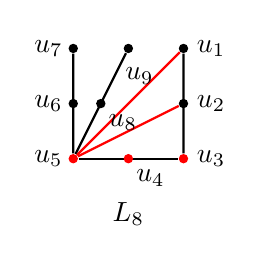
\begin{tikzpicture}[scale=0.7, every node/.style={circle, fill, inner sep=1.2pt}]
	\node[fill=red] (v1) at (-1, 0) {};

	\node[fill=red] (v3) at (1, 0) {};
	\node[fill=black] (v4) at (-1, 1) {};
	\node[fill=black] (v5) at (-1, 2) {};
	\node[fill=black] (v6) at (-0.5, 1) {};
	\node[fill=black] (v7) at (0, 2) {};
	\node[fill=black] (v8) at (1, 1) {};
	\node[fill=black] (v9) at (1, 2) {};

	\draw[black, thick] (v1) -- (v3);
	\draw[black, thick] (v1) -- (v5);
	\draw[black, thick] (v1) -- (v7);
	\draw[black, thick] (v3) -- (v9);
	\draw[red, thick] (v1) -- (v8);
	\draw[red, thick] (v1) -- (v9);
	\node[fill=red] (v2) at (0, 0) {};
	\node[draw=none,fill=none] at (-1.45, 2) {$u_7$};
	\node[draw=none,fill=none] at (-1.45, 1) {$u_6$};
	\node[draw=none,fill=none] at (-1.45, 0) {$u_5$};
	\node[draw=none,fill=none] at (0.4, -0.35) {$u_4$};
	\node[draw=none,fill=none] at (-0.1, 0.65) {$u_8$};
	\node[draw=none,fill=none] at (0.2, 1.5) {$u_9$};
	\node[draw=none,fill=none] at (1.5, 2) {$u_1$};
	\node[draw=none,fill=none] at (1.5, 1) {$u_2$};
	\node[draw=none,fill=none] at (1.5, 0) {$u_3$};
	\node[draw=none,fill=none] at (0, -1) {$L_8$};
\end{tikzpicture}	
\end{figure}

Let $S = \{u_6, u_7, u_8, u_9\}$. By linearity, $E_3(S)=\emptyset$. For any edge $h$ in $E_2(S)$, let $\tilde{u}=h-S$. If $\tilde{u}\in V$, then $u_1u_2u_3,u_3u_4u_5,u_5u_6u_7,h$ and an edge in $E_3(V)$ form a $P_5$, a contradiction. If $\tilde{u}\notin\{u_3,u_4,u_5\}$, then there is a $L_{11}$ consisting of $h,u_7u_6u_5,u_5u_8u_9$ and $u_5u_3u_4$, which is disjoint from $V$, contradicting (2). If $\tilde{u}\in\{u_3,u_4\}$, there is still a $L_{11}$ or $L_{12}$, consisting of $h,u_7u_6u_5,u_5u_3u_4$ and $u_1u_2u_3$, which is disjoint from $V$, contradicting case (2) or case (3). So $E_2(S)\subseteq\{u_5u_6u_7,u_5u_8u_9\}$.

For any edge $g$ in $E_1(S)$, if $g\cap V=\emptyset$, it is easy to find a $P_4,C_4,L_{11}$ or $L_{12}$ disjoint from $V$, contradicting~\Cref{4P2}, case (2) or case (3). Thus $g$ connects $V$ and $U$. However, vertices in $S$ are not 2-centers or vertices of center pairs, so by~\Cref{conpath}, $v_3\in g$. Further, $g-\{v_3\}\cup S\in\{u_3,u_4\}$, or we can easily find a $P_5$ in $G$, a contradiction. So by linearity, $|E_1(S)|\le 2$, and thus $|E(S)|\le 4<\frac{15}{11}|S|$, contradicting~\Cref{contradiction}.\\
    
	(5) $U=L_{13}$.
    \begin{figure}[h]
	\centering
	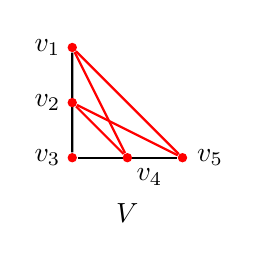
\begin{tikzpicture}[scale=0.7, every node/.style={circle, fill, inner sep=1.2pt}]
		\node[fill=red] (v1) at (-1, 0) {};
		\node[fill=red] (v3) at (1, 0) {};
		\node[fill=red] (v5) at (-1, 2) {};
		
		\draw[black, thick] (v1) -- (v3);
		\draw[black, thick] (v1) -- (v5);
        \node[fill=red] (v4) at (-1, 1) {};
		\node[fill=red] (v2) at (0, 0) {};
        
		\draw[red, thick] (v3) -- (v4);
		\draw[red, thick] (v2) -- (v5);
		\draw[red, thick] (v3) -- (v5);
		\draw[red, thick] (v2) -- (v4);

		\node[draw=none,fill=none] at (-1.45, 2) {$v_1$};
		\node[draw=none,fill=none] at (-1.45, 1) {$v_2$};
		\node[draw=none,fill=none] at (-1.45, 0) {$v_3$};
		\node[draw=none,fill=none] at (0.4, -0.35) {$v_4$};
		\node[draw=none,fill=none] at (1.5, 0) {$v_5$};
		\node[draw=none,fill=none] at (0, -1) {$V$};
		
	\end{tikzpicture}%
    \hspace{0.4cm}
	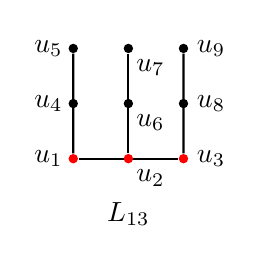
\begin{tikzpicture}[scale=0.7, every node/.style={circle, fill, inner sep=1.2pt}]
	\node[fill=red] (v1) at (-1, 0) {};
	\node[fill=red] (v3) at (1, 0) {};
	\node[fill=black] (v4) at (-1, 1) {};
	\node[fill=black] (v5) at (-1, 2) {};
	\node[fill=black] (v6) at (0, 1) {};
	\node[fill=black] (v7) at (0, 2) {};
	\node[fill=black] (v8) at (1, 1) {};
	\node[fill=black] (v9) at (1, 2) {};
	
	\draw[black, thick] (v1) -- (v3);
	\draw[black, thick] (v1) -- (v5);

	\draw[black, thick] (v3) -- (v9);
	\node[fill=red] (v2) at (0, 0) {};
	\draw[black, thick] (v2) -- (v7);
	\node[draw=none,fill=none] at (-1.45, 2) {$u_5$};
	\node[draw=none,fill=none] at (-1.45, 1) {$u_4$};
	\node[draw=none,fill=none] at (-1.45, 0) {$u_1$};
	\node[draw=none,fill=none] at (0.4, -0.35) {$u_2$};
	\node[draw=none,fill=none] at (0.4, 0.65) {$u_6$};
	\node[draw=none,fill=none] at (0.4, 1.65) {$u_7$};
	\node[draw=none,fill=none] at (1.5, 2) {$u_9$};
	\node[draw=none,fill=none] at (1.5, 1) {$u_8$};
	\node[draw=none,fill=none] at (1.5, 0) {$u_3$};
	\node[draw=none,fill=none] at (0, -1) {$L_{13}$};
\end{tikzpicture}	
\end{figure}

Let $S = \{u_4, u_5, u_6, u_7, u_8, u_9\}$.	By~\Cref{4P2}, $E_3(S)= \emptyset$. For any edge $h\in E_2(S)$, let $\tilde{u}=h-S$. If $\tilde{u}\in V$, there is a $P_5$ consisting of three edges in $U$, the edge $h$ and one edge in $V$. If $\tilde{u}\notin V$, there is a $P_4$ disjoint from $V$, contradicting~\Cref{4P2}.  
Similarly to avoid presence of $P_4$ or $C_4$ disjoint from $V$, for any edge $g\in E_1(S)$, $g$ must connect $V$ and $U$. Moreover, by~\Cref{conpath}, $v_3\in g$. Finally, the vertex $g-\{v_3\}\cup S\in\{u_1,u_2,u_3\}$, or we can find a $P_5$ in $G$, a contradiction. So by linearity, $|E_1(S)|\le 3$ and thus $|E(S)|\le 6<\frac{15}{11}|S|$, contradicting~\Cref{contradiction}.
\end{proof}

\end{document}
